\chapter{Fazit}

Fazit: Ziel unserer Simulation war es, den maximalen gesamten Verkehrsfluss auf beiden Straßen zu bestimmen. Dazu wollen wir den gesamten Fluss bestimmen, dies ist einfach die Summe aus den beiden einzelnen Verkehrsflüssen.\\

Der Verkehrsfluss der horizontalen Straße hängt im wesentlichen von der Dichte der vertikalen Straße ab, da die Autos an der Kreuzung warten müssen bis die Rechts vor Links Regel ihnen frei Fahrt gibt. Aus \cite{book:bungartz} ist bekannt, dass für eine einfache Ringstraße der Verkehrsfluss für eine Dichte von $\rho_max \approx 0.12$ maximal ist, dabei ist der Fluss $f \approx 3000$ Autos pro Stunde. Außerdem können wir aus dieser Quelle entnehmen, dass realistische Verkehrsbedingungen mit einer Trödelwahrscheinlickeit von $p=0.2$ erreicht werden. Deshalb haben wir im Folgenden die horizontale Dichte $\rho_v$ auf den Wert $0.12$ festgesetzt und sind von einer Trödelwahrscheinlichkeit $0.2$ ausgegangen. 
%
\begin{figure}[h]%
\centering
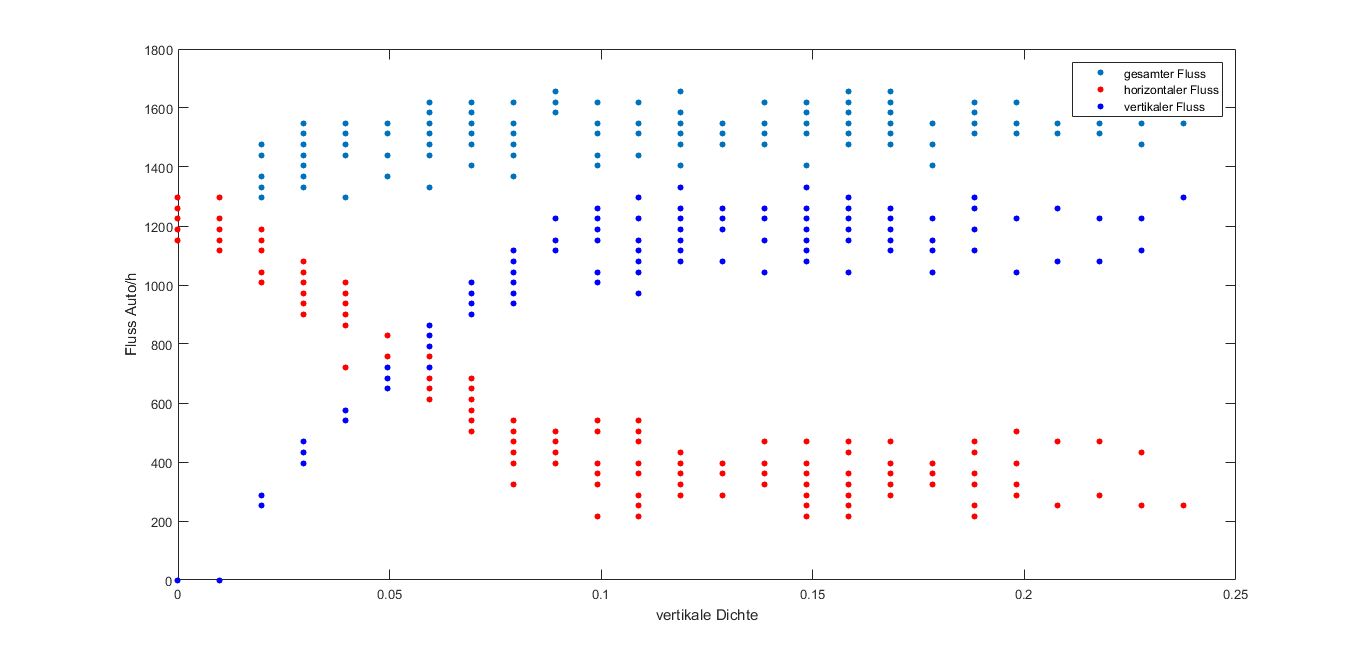
\includegraphics[width=17cm]{MaxFluss.png}%
\caption{Die verschiedenen Flüsse für $p=0.2$, $rho_h=0.12$ und einer Straßenlänge von je 300 Zellen.  }%
\label{pic:MaxFluss}%
\end{figure}
%
In der Abbildung \ref{pic:MaxFluss} sind die einzelnen Flüsse in einer Grafik dargestellt. Man kann erkennen, dass sich der gesamte Fluss ab einer Dichte $\rho_v =0.05$ im wesentlichen Konstant auf einem Niveau von ca. 1500 Autos pro Stunde hält. Ein Grund für diese Erscheinung ist die Bedingung, dass sich beide Ringstraßen eine Zelle, nämlich die Kreuzungszelle teilen. Dadurch wird der Fluss begrenzt. Durch das Abbremsen vor der Kreuzung wird auch die Geschwindigkeit auf der Kreuzung limitiert, so kann ein Auto nur mit geringer Geschwindigkeit über die Kreuzung fahren. Dies beschränkt auch den maximal möglichen Fluss.

Erhöht man die Dichte der vertikalen Straße erhöht sich zwar der vertikale Fluss, aber dafür reduziert sich der horizontale Fluss im gleichen Maße. Bei einer vertikalen Dichte von ungefähr $0.05$ ist der Verkehrsfluss auf beiden Straßen identisch, obwohl die horizontale Dichte mehr als doppelt so hoch ist.

Ausblick:\\
TODO mögliche Erweiterungen wie Ampel oder mehr Kreuzungen oder Abbiegen etc.
